%----------------------------------------------------------------
%
%  File    :  survey-JS.tex
%
%  Author  :  Helmut Zöhrer, TU Graz, Austria
% 
%  Created :  01 Dec 2016
% 
%  Changed :  06 Dec 2016
% 
%----------------------------------------------------------------


\chapter{JavaScript (JS)}

\label{chap:JS}

As an addition to plain CSS, animations can also be brought to life via 
JavaScript (JS) or a combination of CSS and JS. When to use which kind of 
implementation method is dependent on the possibilities in terms of control and 
effect one wants to achieve. 

\section{When to Use JS Instead of CSS}

As a rule of thumb, JS should not be used if the same effect could be achieved 
with plain CSS. This is due to performance and resource management reasons. 
Just when CSS is stretched to its limits, JS should be used. There is a rough 
distinction whether to use CSS or JS for particular kinds of tasks:
\begin{itemize}
	\item Use CSS animations for simple transitions, like changing the 
state of a UI element.
	\item Use JS animations to get advanced effects like bouncing, stop, 
pause, rewind, or slow down (there is more control over animations).
	\item When choosing to animate with JS, considering using the Web 
Animations API or a modern framework (comfortable to work with) may be 
desirable.
\end{itemize}
Apart from this clear distinction, using both CSS and JS works also well. One 
could perform animations with CSS and control states with JS.
\citep{googleDev}

\section{Examples of Useful Animations with JS}

The following example taken from \citet{transformsJS} is capable of breaking 
the CSS-habit of isolating transformations such as scaling, rotations and 
transposing. To be more precise, this example allows independent animations at 
a time with the help of partially overlapping start and ending times as well as 
different easing effects. This example would not be implementable with pure CSS.

\begin{lstlisting}[
language=JavaScript,
label=transformJS,
caption={[Independent Transformations (Rotation, Position) with JS]%
This example shows independent transformations, such as scaling, rotating and 
changing the position of some text.
}
]
//pulsate the box using scaleX and scaleY
TweenMax.to($box, 1.2, {scaleX:0.8, scaleY:0.8, force3D:true, yoyo:true, 
repeat:-1, ease:Power1.easeInOut});

$("#rotation").click(function() {
rotation += 360;
TweenLite.to($box, 2, {rotation:rotation, ease:Elastic.easeOut});
});

$("#rotationX").click(function() {
rotationX += 360;
TweenLite.to($box, 2, {rotationX:rotationX, ease:Power2.easeOut});
});

$("#rotationY").click(function() {
rotationY += 360;
TweenLite.to($box, 2, {rotationY:rotationY, ease:Power1.easeInOut});
});

$("#move").click(function() {
if (wanderTween) {
wanderTween.kill();
wanderTween = null;
TweenLite.to($box, 0.5, {x:0, y:0});
} else {
wander();
}
});

//randomly choose a place on the screen and animate there, then do it again, 
and again.
function wander() {
var x = (($field.width() - $box.width()) / 2) * (Math.random() * 1.8 - 0.9),
y = (($field.height() - $box.height()) / 2) * (Math.random() * 1.4 - 0.7);
wanderTween = TweenLite.to($box, 2.5, {x:x, y:y, ease:Power1.easeInOut, 
onComplete:wander});
}
\end{lstlisting}

\label{list:transformJS}


Another example (\citet{imposJS}) which uses the combined power of CSS and JS 
is the following. Some random text is animated with a lively turn-around 
effect. It is based on the ability to split up stings into separate characters 
via JS.


\begin{lstlisting}[
language=JavaScript,
label=imposJS,
caption={[Performing Turn-around Effect in JS]%
This example implements a turn-around effect of text with the help of splitting 
up strings into single characters and animating them individually.
}
]
tl = new TimelineLite({onUpdate:updateSlider, onComplete:onComplete, 
onReverseComplete:onComplete, paused:true});

//do a simple split of the text so we can animate each character (doesn't 
require the advanced features of SplitText, so we just use split() and join())
$text.html("<span>" + 
$text.html().split("").join("</span><span>").split("<span> 
</span>").join("<span>&nbsp;</span>") + "</span>");

//set a perspective on the container
TweenLite.set($text, {perspective:500});

//all of the animation is created in this one line:
tl.staggerTo($("#text span"), 4, {transformOrigin:"50% 50% -30px", 
rotationY:-360, rotationX:360, rotation:360, ease:Elastic.easeInOut}, 0.02);
}
\end{lstlisting}


\begin{figure}[tp]
\centering
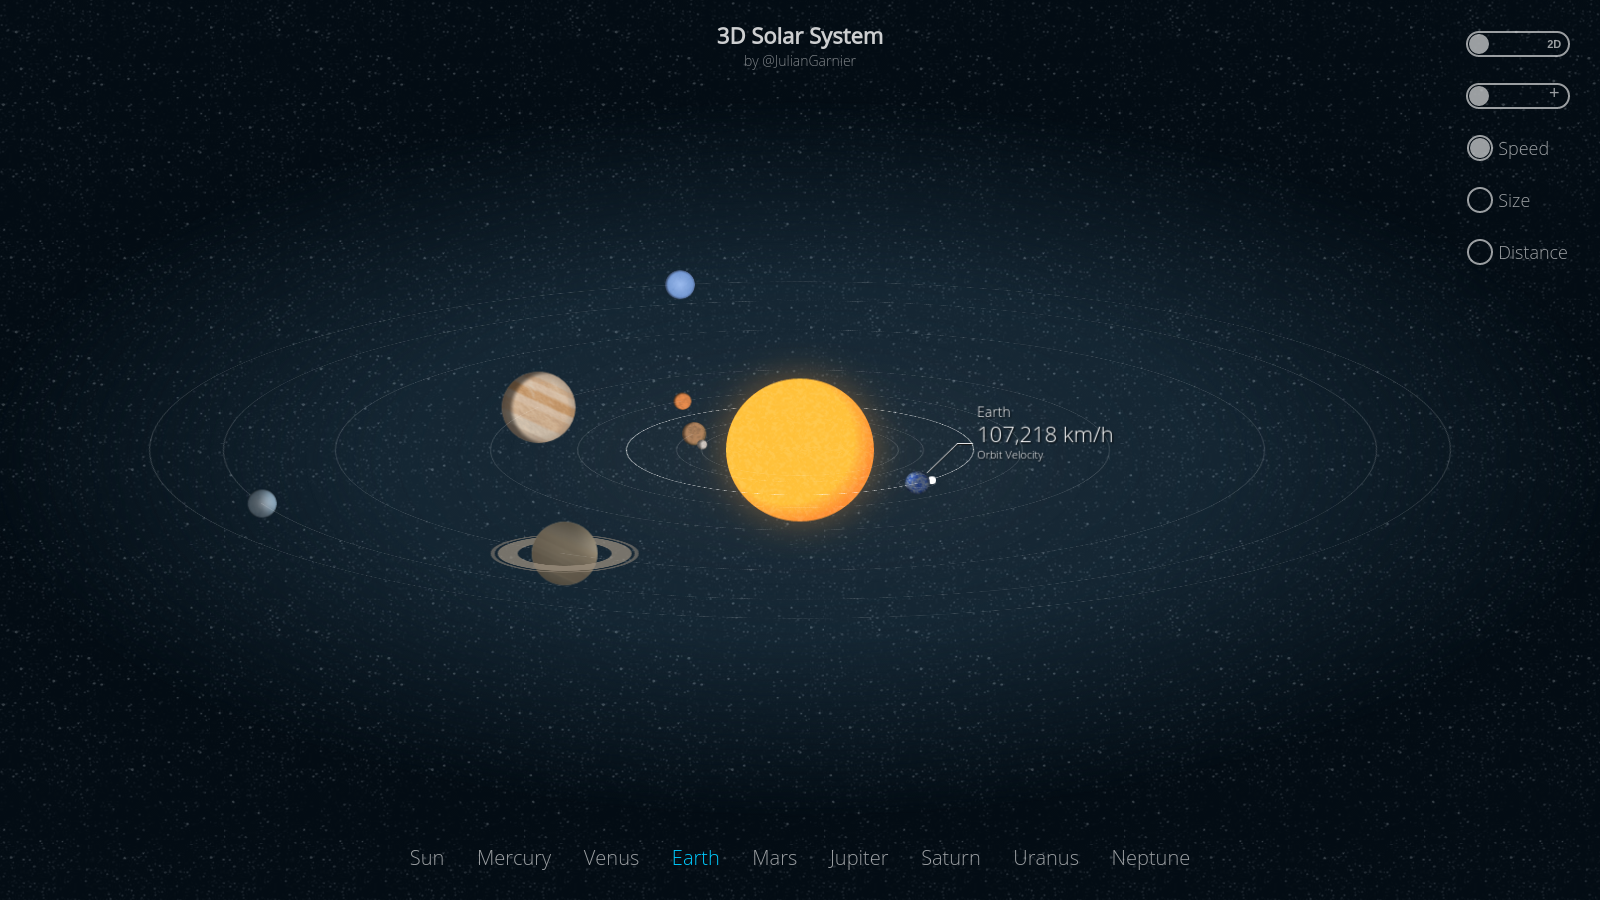
\includegraphics[keepaspectratio,scale=0.25]{images/solar.png}
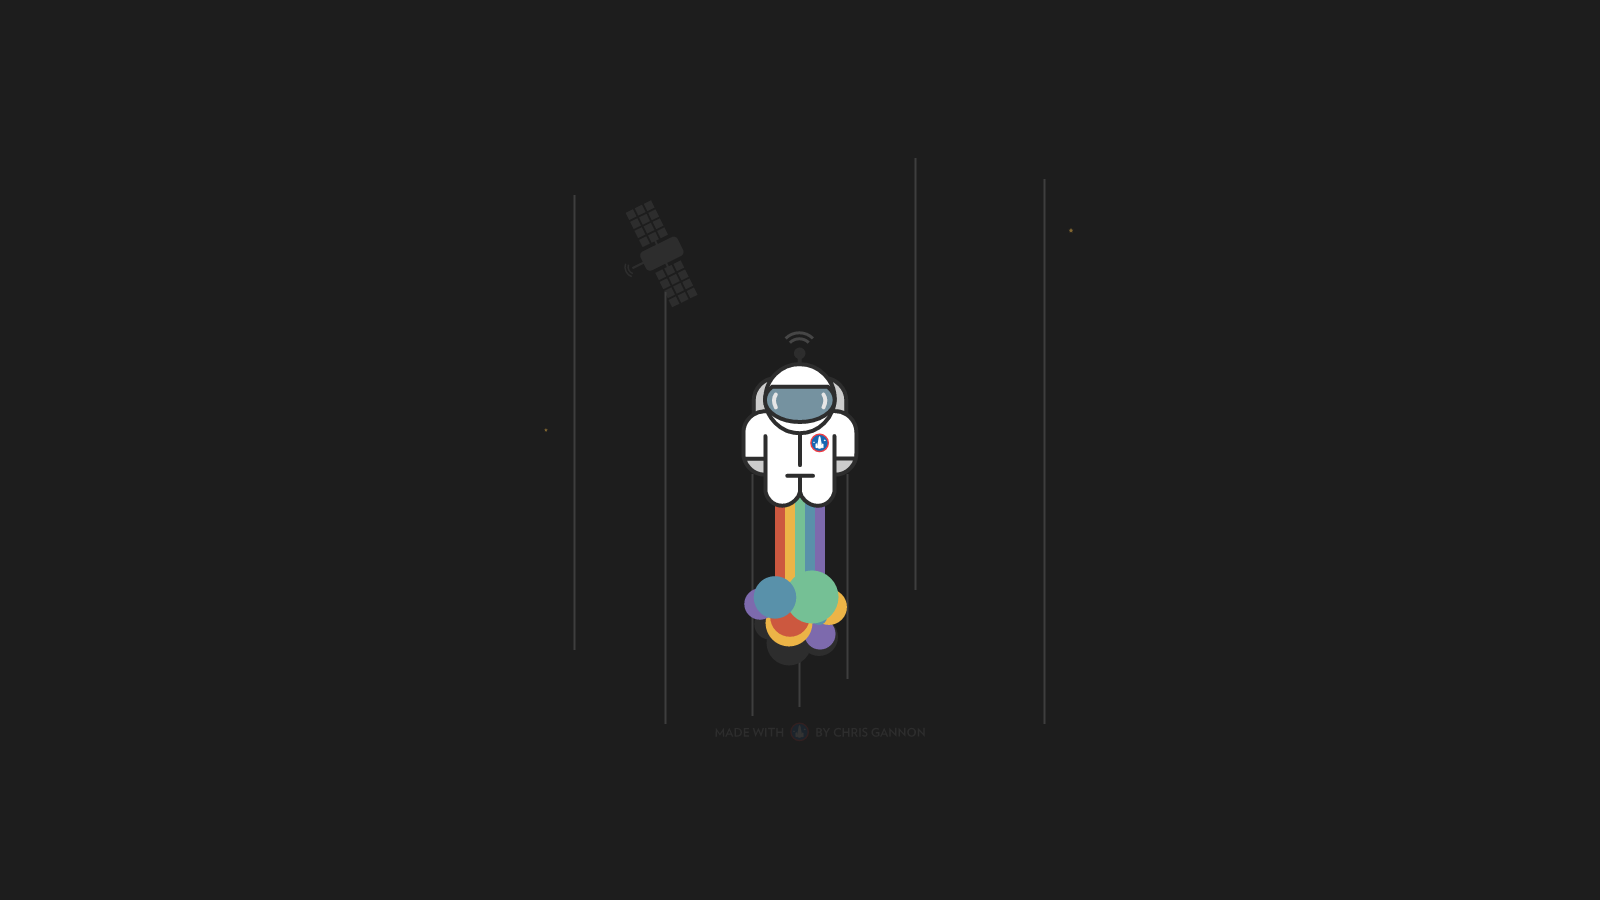
\includegraphics[keepaspectratio,scale=0.25]{images/rocketman.png}

\caption[Powerful JavaScript Examples]{
We provide also great animation examples of combining CSS and JS in code 
folders solar and rocketmanSVG, to show the potential we can achieve. While the 
solar system at the top is purely CSS and JS, the bottom rocketman uses SVG 
with CSS and JS to draw more complex objects. This are not so much animations 
directed at UI development as simulations, however they greatly show the 
possibilities of CSS and JS for animation.
\imgcredit{Screenshot taken by the authors of this survey. The code behind the 
pages is by using the \citet{solarSystem,rocketmanSVG} online snippets.}
}
\label{fig:powerfulJS}
\end{figure}


\label{list:imposJS}